
\paragraph{3. Presence of cycles?}
    Before we go into analyzing whether new relations introduce observable behaviours, we first ensure there are no $\stck{_\textit{hb}}$ cycles introduced in the process. Consider the example below
    \begin{figure}[H]
        \centering
        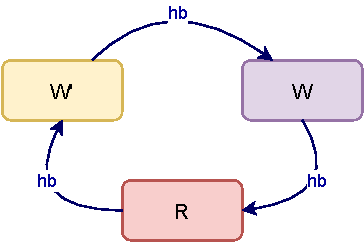
\includegraphics[scale=0.7]{InstructionReordering/ValidReorderingProof/ProofParts/Part3/part3(a).pdf}
        \caption{Caption}
        \label{fig:my_label}
    \end{figure}

    Notice that here, the axiom of coherent reads restricts $R$ to read from $W'$.
    \[
        \reln{R}{hb}{W'} \Rightarrow \neg \reln{R}{rf}{W'}
    \]

    But by transitive property, it is also the case that $\reln{W'}{hb}{R}$. 
    \[
        \reln{W'}{hb}{W} \ \wedge \ \reln{W}{hb}{R} \ 
        \Rightarrow \ 
        \reln{W'}{hb}{R}
    \]

    As per this, the axiom of coherent reads shouldn't restrict $\reln{R}{rf}{W'}$. To avoid such cases, we will need to ensure that no Candidate Execution of $C'$ after $e$ and $d$ are reordered have $\stck{_{hb}}$ cycles.

    Note that if a cycle exists after reordering, then 
    \begin{enumerate}
        \item The relations preserved do not themselves create a cycle (ref to the theorem)
        \item Additional new relations may introduce cycles
    \end{enumerate}

    The first part is straightforward as we assume we can only do reordering on Candidate Exectuions of $C$ not having happens-before cycles. 

    For the second part, we first address the cases where $\reln{d}{hb}{e}$ may be part of the cycle. The other event $k$, may be either from the set $K_e$, $K_d$ or a new relation that is formed.

    \critic{blue}{$K_e$ and $K_d$ only apart from the new relation because these are the only valid cases where happens-before relations are preserved after reordering. So we need not consider cases such thta $\reln{e}{hb}{k}$ or $\reln{k}{hb}{d}$ as the old relationsas they are covered by $K_e$ and $K_d$.}
    %Show figure here
    \begin{figure}[H]
        \centering
        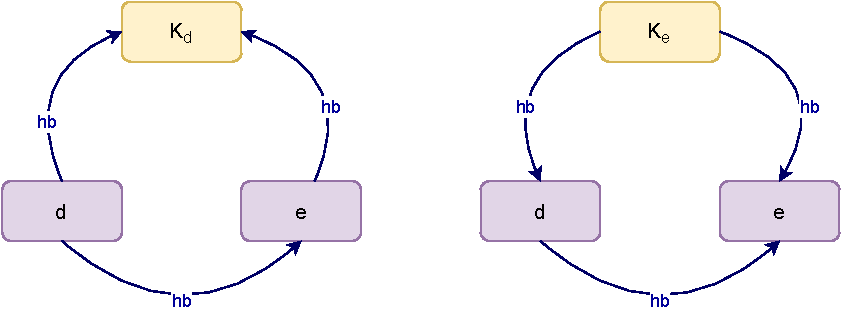
\includegraphics[scale=0.7]{InstructionReordering/ValidReorderingProof/ProofParts/Part3/part3(b).pdf}
        \caption{If k belongs to one of the sets $K_e$ or $K_d$}
        \label{fig:my_label}
    \end{figure}

    The above figure shows that $k$ cannot belong to either of the sets, as their relations with $e$ and $d$ will not result in a cycle. 

    For cases where $\reln{k}{hb}{e}$ is the set of new relations, note that by lemma 1
    \[
        \reln{k}{hb}{e} \Rightarrow \reln{k}{hb}{d}
    \]

    For cases where $\reln{d}{hb}{k}$ is the set of new relations, by lemma 2
    \[
        \reln{d}{hb}{k} \Rightarrow \reln{e}{hb}{k}
    \]

    So for both these cases also, a cycle with $\reln{d}{hb}{e}$ cannot exist. The following figure shows pictorially this fact. 
    %Show figure here
    \begin{figure}[H]
        \centering
        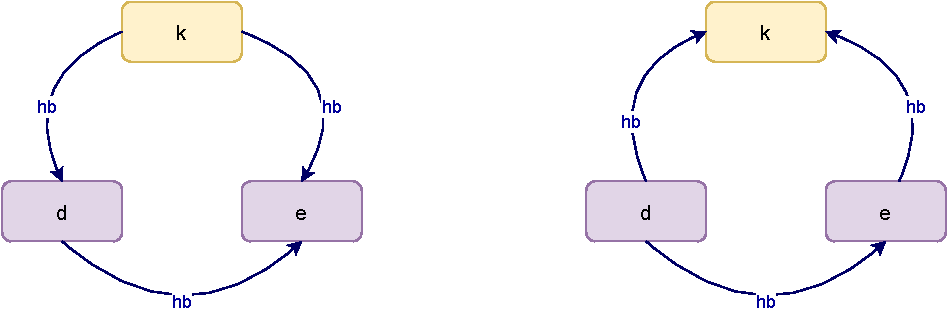
\includegraphics[scale=0.7]{InstructionReordering/ValidReorderingProof/ProofParts/Part3/part3(c).pdf}
        \caption{If $\reln{k}{hb}{e}$ or $\reln{d}{hb}{k}$ are new sets of relations}
        \label{fig:my_label}
    \end{figure}

    For the one case where we have two new sets of relations formed, i.e $\reln{d}{hb}{k}$ and $\reln{k}{hb}{e}$, we could have a case where $k$ is a common event for both sets. But, by lemma 1, we also have $\reln{k}{hb}{d}$ and by lemma 2, $\reln{e}{hb}{k}$. Thus, we have a cycle. The following figure shows this pictorially

    %Show figure here
    \begin{figure}[H]
        \centering
        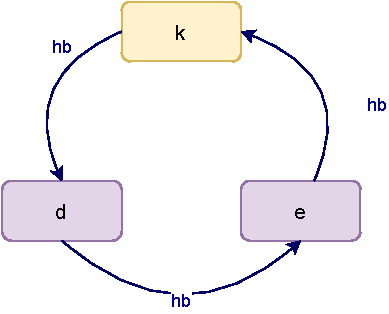
\includegraphics[scale=0.7]{InstructionReordering/ValidReorderingProof/ProofParts/Part3/part3(d).pdf}
        \caption{A cycle exists in the case where we have two new sets of relations ($\reln{k}{hb}{e}$ and $\reln{d}{hb}{k}$) }
        \label{fig:my_label}
    \end{figure}

    \critic{blue}{It is not actually due to lemmas, but just that the new relations were derived through $e$ or $d$, as these relations existed before reordering.}

    \critic{purple}{Maybe have a better figure, meaning a set of relations where each figure shows clearly which relaiton is implied due to whcih lemma}

    Now for the case when $\reln{d}{hb}{e}$ may not be part of the cycle, we have only two other new relations, $\reln{k}{hb}{e}$ or $\reln{d}{hb}{k}$.

    Considering the first scenario where the new set of relations are of the form $\reln{k}{hb}{e}$. Suppose a cycle exists with another event $k'$. Then 
    \[
        \reln{k}{hb}{e} \ \wedge \
        \reln{e}{hb}{k'} \ \wedge \
        \reln{k'}{hb}{k}
    \]

    Note that the latter two relations are not new, since the only new set of relations are of the first form. Now, by lemma 1 and by transitivity respectively
    \begin{gather*}
        \reln{k}{hb}{e} \Rightarrow \reln{k}{hb}{d} \\
        \reln{e}{hb}{k'} \Rightarrow \reln{d}{hb}{k'}    
    \end{gather*}

    So, the following is also a cycle
    \[
        \reln{k}{hb}{d} \ \wedge \
        \reln{d}{hb}{k'} \ \wedge \
        \reln{k'}{hb}{k}
    \]

    But these relations already exist in the original Candidate Execution, which implies a cycle existed before reordering. This contradicts our assumption that we only reorder when the Candidate Executions of $C$ have no cycles. Thus, by contradiction such a cycle cannot exist.

    In similar lines for the cases where the set of new relations are of the form $\reln{d}{hb}{k}$, we can show by contradiction that a cycle cannot exist.
